\documentclass[border=10pt]{standalone}
\usepackage{tikz}
\usetikzlibrary{arrows.meta, shapes, calc}

\begin{document}
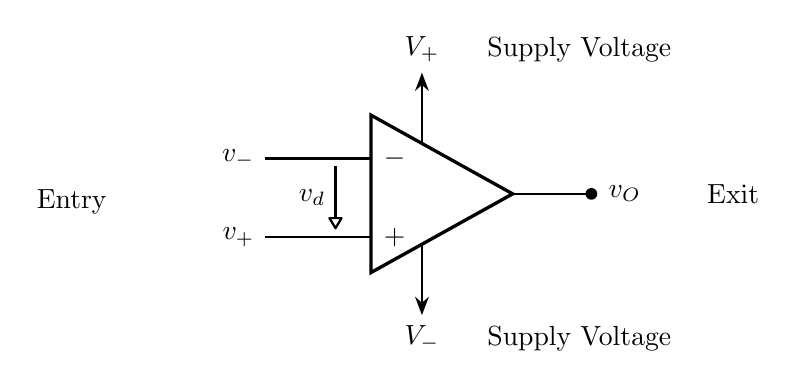
\begin{tikzpicture}[thick, >=Stealth]

% Define coordinates for the op-amp triangle
\coordinate (A) at (0,0);
\coordinate (B) at (0,2);
\coordinate (C) at (1.8,1);
\coordinate (InMinus) at (0,1.45);
\coordinate (InPlus) at (0,0.45);
\coordinate (VPlusTap) at ($(B)!0.36!(C)$);
\coordinate (VMinusTap) at ($(A)!0.36!(C)$);

% Draw the op-amp triangle
\draw[very thick] (A) -- (B) -- (C) -- cycle;

% Draw input lines
\draw (InMinus) -- ++(-1.35,0) node[left] {$v_-$};
\draw (InPlus) -- ++(-1.35,0) node[left] {$v_+$};

% Draw differential voltage arrow
\draw[-{Triangle[round,open]}] (-0.45,1.35) -- (-0.45,0.55) node[midway, left] {$v_d$};

% Draw output line
\draw (C) -- ++(1,0) node[circle, fill, inner sep=1.5pt, label=right:{$v_O$}] (Out) {};
\node at (4.6,1) {Exit};

% Draw supply voltage lines
\draw[->] (VPlusTap) -- ++(0,0.9) node[above] (VPlus) {$V_+$} node[right=0.7cm] at (VPlus) {Supply Voltage};
\draw[->] (VMinusTap) -- ++(0,-0.9) node[below] (VMinus) {$V_-$} node[right=0.7cm] at (VMinus) {Supply Voltage};

% Draw input labels
\node at (0.3,1.45) {$-$};
\node at (0.3,0.45) {$+$};

% Draw "Entry" label
\node at (-3.8,0.9) {Entry};

\end{tikzpicture}
\end{document}
